\documentclass[mathserif]{beamer}
\usepackage{beamerthemeshadow}
\usepackage{beamerthemesplit}
%\usetheme{shadow}
\usecolortheme{lily}
%\usepackage{amsmass}
%\usepackage{amssymb,amsfonts,url}

\usepackage{algorithm}
\usepackage{algorithmic}
\usepackage{graphicx}

\graphicspath{{Problems/}}

\usepackage{tikz}
\usetikzlibrary{shadows}
\usetikzlibrary{positioning}
\usepackage{verbatim}
\usepackage{pgfplots}
\usepackage{verbatim}
\usetikzlibrary{arrows,shapes}

\definecolor{darkblue}{rgb}{0.2,0.2,0.6}
\definecolor{darkred}{rgb}{0.6,0.1,0.1}
\definecolor{darkgreen}{rgb}{0.2,0.6,0.2}

\usetikzlibrary{shadings,shadows,shapes.arrows}

\usetikzlibrary{calc} 
\makeatletter 
\@namedef{color@3}{blue!20}
\@namedef{color@1}{green!70}   
%\@namedef{color@3}{yellow!50} 
\@namedef{color@2}{orange!90}  
%\@namedef{color@5}{magenta!70} 
%\@namedef{color@6}{yellow!70}    0

\newcommand{\graphitemize}[2]{%
\begin{tikzpicture}[every node/.style={align=center}, scale=0.78]  
 \draw[fill=green!5, fill opacity=0.1, green, inner sep=0.05cm, outer sep=0.05cm] (5,0) arc(0:360:5);
 % \draw[fill=white, fill opacity=0.1, white, inner sep=0.05cm, outer sep=0.05cm] (4,0) arc(0:360:4);
%  \shade[ball color=gray!10!] (0,0) coordinate(Hp) circle (.9);
  \node[shape=circle,  minimum size=1.1cm,fill=blue!20!60,fon$i=$\Large,outer sep =.15cm,inner sep=.2cm,drop  shadow={ashadow, color=yellow}](ce){#1};  
   % \shade[ball color=blue!20!] (0,0) coordinate($Algorithm$) circle (1.5cm);

\foreach \gritem [coun$i=$\xi] in {#2}  {\global\let\maxgritem\xi}  
\foreach \gritem [coun$i=$\xi] in {#2}
{% 
\pgfmathtruncatemacro{\angle}{90+360/\maxgritem*\xi}
\edef\col{\@nameuse{color@\xi}}
\node[shape=circle,
     ultra thick,
     draw=white,
     fill opacity=1,
     drop  shadow={ashadow, color=blue!60},
     fill=\col,outer sep=0.25cm,        
     minimum size=2cm] (satellite-\xi) at (\angle:5cm) {\gritem };
     \draw[line width=0.25cm,-latex, \col] (ce) -- (satellite-\xi);
     }%
% \draw[violet, fill=violet!10] (4,0) arc(0:360:4);
\end{tikzpicture}  
}%



\newcommand*{\tikzarrow}[2]{%
  \tikz[
    baseline=(A.base),             % Set baseline to the baseline of node content
    fon$i=$\footnotesize\sffamily    % Set fontsize of the node content
  ]
  \node[
    single arrow,                  % Shape of the node
    single arrow head extend=2pt,  % Actual width of arrow head
    draw,                          % Draw the node shape
    inner sep=2pt,                 % Separation between node content and node shape
    top color=white,               % Shading color on top of node
    bottom color=#1,               % Shading color on bottom of node
    drop shadow                    % Draw a shadow
  ] (A) {#2};%
}


\def\arrow{
  (10.05:1.1) -- (6.05:1) arc (6.05:120:1) [rounded corners=0.5] --
  (120:0.9) [rounded corners=1] -- (130:1.1) [rounded corners=0.5] --
  (120:1.3) [sharp corners] -- (120:1.2) arc (120:5.25:1.2)
  [rounded corners=1] -- (10.05:1.1) -- (6.05:1) -- cycle
}

\tikzset{
  ashadow/.style={opacity=.25, shadow xshif$i=$0.07, shadow yshif$i=$-0.07},
}

\def\arrows[#1]{         
  \begin{scope}[scale=#1]
    \draw[color=darkred, drop  shadow={ashadow, color=red!60!black}] \arrow;

    \draw[color=darkgreen, bottom color=green!90!black, top color=green!60,   drop shadow={ashadow, color=green!60!black}] [rotate=120] \arrow;

    \draw[color=darkblue, right color=blue, left color=blue!60,   drop shadow={ashadow, color=blue!60!black}] [rotate=240] \arrow;

    % to hide the green shadow
    \draw[color=darkred, left color=red, right color=red!60] \arrow;
  \end{scope}
}

\tikzstyle{vertex}=[circle,fill=black!25,draw,minimum size=20pt,inner sep=0pt]
\tikzstyle{middlevertex}=[circle,fill=black!25,draw,minimum size=15pt,inner sep=0pt]
\tikzstyle{smallvertex}=[circle,fill=black!25,draw,minimum size=10pt,inner sep=0pt]
\tikzstyle{tinyvertex}=[circle,fill=black!25,draw,minimum size=5pt,inner sep=0pt]
\tikzstyle{selected vertex} = [vertex, draw,fill=yellow!24]
\tikzstyle{blue smallvertex} = [smallvertex, draw,fill=blue!20]
\tikzstyle{red smallvertex} = [smallvertex, draw,fill=yellow]
\tikzstyle{edge} = [draw,thick,->]
\tikzstyle{undirectededge} = [draw,thick]
\tikzstyle{weight} = [fon$i=$\small]
\tikzstyle{selected edge} = [draw,line width=3pt,-,red!50]
\tikzstyle{ignored edge} = [draw,line width=3pt,-,black!20]
\tikzstyle{squarednode}=[draw, fill=blue!20, thick, minimum size=5mm]
\tikzstyle{roundnode}=[circle, draw, fill=blue!20, thick, minimum size=5mm]

\usetikzlibrary{arrows,automata}


%\usepackage{CJK}
%\usepackage{pinyin}

%    \begin{figure}
%        \centering
%        \includegraphics[width=0.8\textwidth]{newGeneRep.png
%}
%    \end{figure}

% \begin{figure}%
%   \begin{center}%
%     \begin{minipage}{0.70\textwidth}%
%      \includegraphics[width=1.0\textwidth]{comp25000.png
%}%
%     \end{minipage}%
%     \begin{minipage}{0.30\textwidth}
%      \includegraphics[width=1.0\textwidth]{comparelabel.png
%}%
%     \end{minipage}%
%   \end{center}
% \end{figure}

% \begin{table}
%   {\begin{tabular}{l|rrr}\hline
%       & \multicolumn{3}{c}{Actual number of DCJ operations}\\
%       \# genes &\# genes $\times 1$&\# genes $\times 2$&\# genes  $\times 3$ \\
% \hline
%      (a)~25,000 & 0.5\% ~~&  0.9\% ~~& 1.7\%~~\\
%       (b)~10,000 & 0.8\%~~ &  1.4\% ~~& 2.7\%~~\\
%      (c)~ 1,000 & 2.7\%~~ & 4.7\%~~ & 14.7\%~~\\ \hline
%     \end{tabular}} {}%
% \end{table}

% \begin{eqnarray}
% T(n) &=&  \sum_{i=1}^n C_i \\
%      &=&  \# PUSH + \#POP \\
%      &<& 2\times \#PUSH \\
%      &<& 2n \\
% \end{eqnarray}


\title{CS711008Z Algorithm Design and Analysis }
\subtitle{ Lecture 6. Hidden Markov model and Viterbi's decoding algorithm}
% \footnote{The slides are prepared based on Lecture 3 of The Design and Analysis of Algorithms (by D. C. Kozen), and Chapter 5 of Algorithm design.  }
\author{Dongbo Bu } 
\institute{{\small Institute of Computing Technology \\ Chinese Academy of Sciences, Beijing, China}}
\date{}


\begin{document}
%\begin{CJK}{UTF8}{cyberbit}

\frame{\titlepage}


%\frame{
%\frametitle{Outline}
%\begin{itemize}
% \item Fourier series
% \item Fourier transformation
% \item Discrete Fourier transformation
% \item FFT: The basic idea of FFT (Fast Fourier Transformation); 
% \item Two viewpoints of FFT: 
% 	\begin{enumerate}
%            \item Converting between time-domain and frequency-domain;
%           \item Efficient way to evaluate and multiply polynomials; 
%      \end{enumerate}
% \item Divide-and-conqueror applies due to the judicious choice of $x$ as root of unity. 
%\end{itemize}
%}
%
%\frame{
%\begin{block}{} 
%Fourier series 
%\end{block}
%}
%
%
%
%\frame{
%\begin{block}{}
% Fourier transformation
%\end{block}
%}
%
%
%\frame{
%\begin{block}{}
%Discrete Fourier Transformation
%\end{block}
%}
%
%
%\frame{
%\begin{block}{}
% Fast Fourier transformation
%\end{block}
%}
%
%\frame{
%\begin{block}{}
%Viewpoint 1: Converting between time-domain and frequency-domain. 
%\end{block}
%}
%
%\frame{
%\frametitle{An example of FFT: touch-tone telephone dialing} 
%
%\begin{figure}
%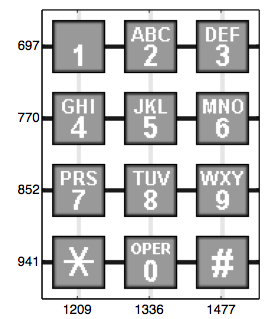
\includegraphics[width=1.5in]{L5-telephonekeypad.png}
%\end{figure} 
%\begin{itemize} 
% \item The basis for touch-tone dialing is the Dual Tone Multi-Frequency. 
%\item When a key is pressed, a tone is generated by superimposing two fundamental tones with different frequency. 
%\end{itemize} 
%} 
%
%\frame{ 
%\frametitle{DFT is used to convert from time-domain to frequency-domain.  } 
%\begin{itemize} 
% \item 
%For example, when $1$ is pressed, the following wave will be observed.
%
%\item Time domain: 
%\begin{figure}
%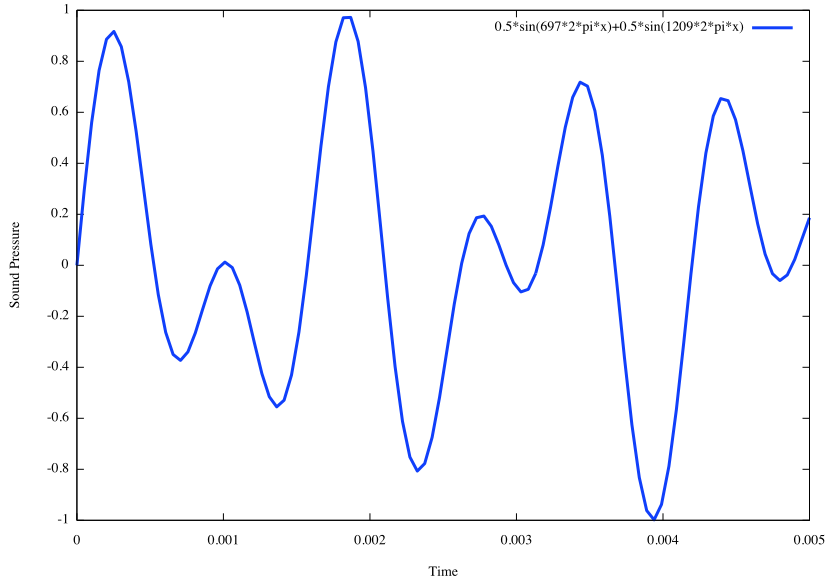
\includegraphics[width=1.3in]{L5-telephonekeypadpress1.png}
%\end{figure} 
%
%\item
%Frequency domain: 
%\begin{figure}
%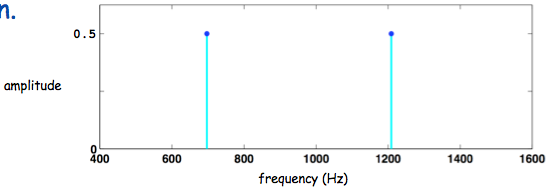
\includegraphics[width=2in]{L5-telephonekeypadpress1fd.png}
%\end{figure} 
%
%\end{itemize} 
%}
%
%
%
%\frame{
%\frametitle{Discrete: acquiring a vector via sampling} 
%
%\begin{itemize}
%\item Sound wave:  
%\begin{figure}
%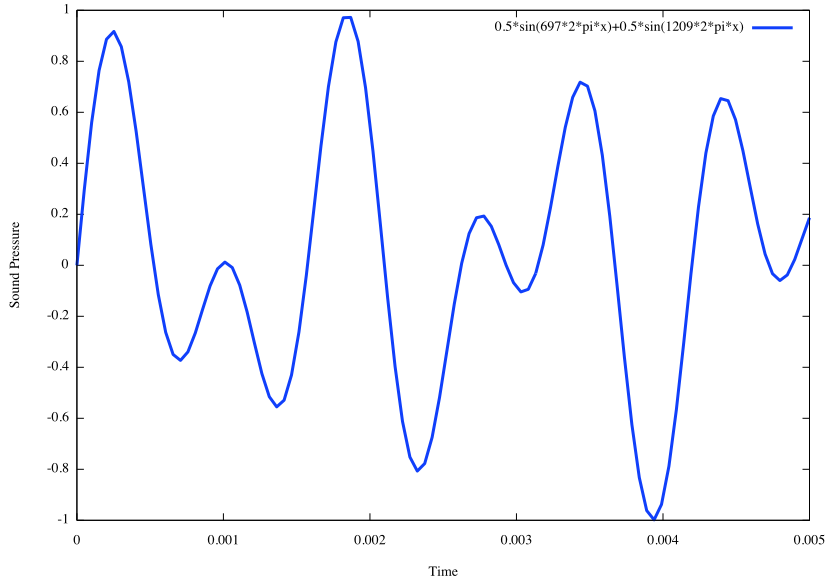
\includegraphics[width=1.5in]{L5-telephonekeypadpress1.png}
%\end{figure} 
%
%\item A vector acquired via sampling: 
%\begin{figure}
%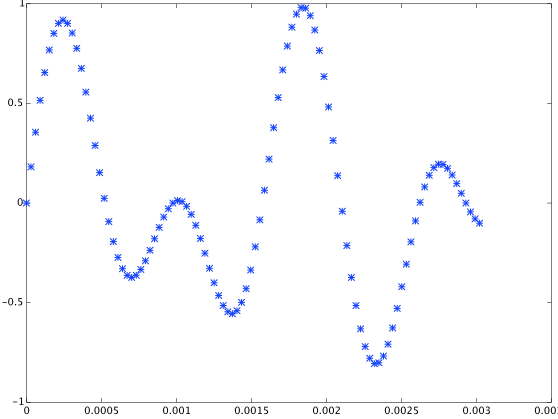
\includegraphics[width=1.5in]{L5-telephonekeypadpress1td.png}
%\end{figure} 
%
%\end{itemize} 
%} 

\frame{
	\frametitle{Outline}
	
	\begin{itemize}
		\item The occasionally dishonest casino: an example of HMM
		\item Formal definition of HMM 
		\item Finding the most probable state path: Viterbi algorithm 
	\end{itemize}
}

\frame{
	\begin{block}{}
		The occasionally dishonest casino: an example of HMM
	\end{block}
}

\frame{
	\frametitle{The occasionally dishonest casino}
	
	\begin{itemize}
		\item A casino have a \textcolor{red}{\bf fair dice} and a \textcolor{red}{\bf loaded dice}. The fair dice has identical probability $\tfrac{1}{6}$ for all numbers one to six while the loaded dice has probability $0.3$ of a five, $0.3$ of a six, and $0.1$ for the numbers one to four. 
		\item For the first roll, the casino uses the fair dice with probability $\tfrac{3}{5}$ and uses the loaded one with probability $\tfrac{2}{5}$. In the subsequent rolls, the casino switches from a fair to a loaded dice with probability $0.2$ and switches back with probability $0.1$. Thus the switch between dice forms a \textcolor{red}{\bf Markov process}.
\begin{figure}
\begin{tikzpicture}[node distance=2cm,->,>=latex,auto,
  every edge/.append style={thick}]
  \node[state, fill=blue!20] (1) {\bf F};
  \node[state, fill=blue!20] (2) [right of=1] {\bf L};  
  \path (1) edge[loop left]  node{\small 0.8} (1)
            edge[bend left]  node{\small 0.2}   (2)
        (2) edge[loop right] node{\small 0.9}  (2)
            edge[bend left] node{\small 0.1}     (1);
            
            
  \def\dx{-3};
 \def\dy{1}; 
 \def\d{0.3}          
  \node[] at (0+\dx, 0+\dy+1*\d) {\small {\bf Fair dice}};
 \node[] at (0+\dx, 0+\dy-1*\d) {\tiny $1:  1/6$};
 \node[] at (0+\dx, 0+\dy-2*\d) {\tiny $2:  1/6$};
 \node[] at (0+\dx, 0+\dy-3*\d) {\tiny $3:  1/6$};
 \node[] at (0+\dx, 0+\dy-4*\d) {\tiny $4:  1/6$};
 \node[] at (0+\dx, 0+\dy-5*\d) {\tiny $5:  1/6$};
 \node[] at (0+\dx, 0+\dy-6*\d) {\tiny $6:  1/6$};
 \draw[thick, blue] (0+\dx - 0.5, 0+\dy+0*\d) rectangle (0+\dx+0.5, 0+\dy-6.5*\d);


 \def\dx{+5};
 \def\dy{1}; 
 \def\d{0.3}          
  \node[] at (0+\dx, 0+\dy+1*\d) {\small {\bf Loaded dice}};
 \node[] at (0+\dx, 0+\dy-1*\d) {\tiny $1:  1/10$};
 \node[] at (0+\dx, 0+\dy-2*\d) {\tiny $2:  1/10$};
 \node[] at (0+\dx, 0+\dy-3*\d) {\tiny $3:  1/10$};
 \node[] at (0+\dx, 0+\dy-4*\d) {\tiny $4:  1/10$};
 \node[] at (0+\dx, 0+\dy-5*\d) {\tiny $5:  3/10$};
 \node[] at (0+\dx, 0+\dy-6*\d) {\tiny $6:  3/10$};
 \draw[thick, blue] (0+\dx - 0.5, 0+\dy+0*\d) rectangle (0+\dx+0.5, 0+\dy-6.5*\d);

           
\end{tikzpicture}
\end{figure}  
	\end{itemize}

}


\frame{
	\frametitle{The occasionally dishonest casino  cont`d}

\begin{figure}
\begin{tikzpicture}[node distance=2cm,->,>=latex,auto,
  every edge/.append style={thick}]
  \node[state, fill=blue!20] (1) {\bf F};
  \node[state, fill=blue!20] (2) [right of=1] {\bf L};  
  \path (1) edge[loop left]  node{\small 0.8} (1)
            edge[bend left]  node{\small 0.2}   (2)
        (2) edge[loop right] node{\small 0.9}  (2)
            edge[bend left] node{\small 0.1}     (1);
            
            
  \def\dx{-3};
 \def\dy{1}; 
 \def\d{0.3}          
  \node[] at (0+\dx, 0+\dy+1*\d) {\small {\bf Fair dice}};
 \node[] at (0+\dx, 0+\dy-1*\d) {\tiny $1:  1/6$};
 \node[] at (0+\dx, 0+\dy-2*\d) {\tiny $2:  1/6$};
 \node[] at (0+\dx, 0+\dy-3*\d) {\tiny $3:  1/6$};
 \node[] at (0+\dx, 0+\dy-4*\d) {\tiny $4:  1/6$};
 \node[] at (0+\dx, 0+\dy-5*\d) {\tiny $5:  1/6$};
 \node[] at (0+\dx, 0+\dy-6*\d) {\tiny $6:  1/6$};
 \draw[thick, blue] (0+\dx - 0.5, 0+\dy+0*\d) rectangle (0+\dx+0.5, 0+\dy-6.5*\d);


 \def\dx{+5};
 \def\dy{1}; 
 \def\d{0.3}          
  \node[] at (0+\dx, 0+\dy+1*\d) {\small {\bf Loaded dice}};
 \node[] at (0+\dx, 0+\dy-1*\d) {\tiny $1:  1/10$};
 \node[] at (0+\dx, 0+\dy-2*\d) {\tiny $2:  1/10$};
 \node[] at (0+\dx, 0+\dy-3*\d) {\tiny $3:  1/10$};
 \node[] at (0+\dx, 0+\dy-4*\d) {\tiny $4:  1/10$};
 \node[] at (0+\dx, 0+\dy-5*\d) {\tiny $5:  3/10$};
 \node[] at (0+\dx, 0+\dy-6*\d) {\tiny $6:  3/10$};
 \draw[thick, blue] (0+\dx - 0.5, 0+\dy+0*\d) rectangle (0+\dx+0.5, 0+\dy-6.5*\d);

           
\end{tikzpicture}
\end{figure}  

\begin{itemize}

%		\item In each state of the Markov process, the outcome of a roll has different probability. Thus, the whole process forms a \textcolor{red}{\bf hidden Markov model}. Here the  \textcolor{red}{\bf state sequence}, i.e. the dice used for each roll,  is hidden. 
		%That is, given a sequence of rolls only, we don't know which rolls used a fair dice and which used the loaded dice, since this is kept secret by casino. 
		\item Question: Suppose we observed a total of $10$ rolls with the following outcomes:
\[
Y = (1, 3, 4, 5, 5, 6, 6, 3, 2, 6)
\]
	Could we find out the most probable state sequence, i.e. the most probable dice used for each roll? 

\end{itemize}
}

\frame{
	\frametitle{Trial 1: Calculating log-odd score based on Markov model} 

	\begin{itemize}
		\item For each observed symbol, we could calculate log-odd score for a window of $w$ rolls around it, and expect the rolls using fair dice to stand out with positive values. 
		\item However, this is unsatisfactory since: 
			\begin{itemize}
				\item This solution  depends heavily on the selection of the window size $w$. 
				\item The rolls generated using fair dice might have sharp boundaries and variable length. 
			\end{itemize}
		\item A better idea is to build a  model to describe the switch between these two dice. 
	\end{itemize}
}

\frame{
	\frametitle{Trial 2: Calculating the most probable state path using HMM} 

\begin{figure}
\begin{tikzpicture}[scale=0.6]

\tikzset{vertex/.style = {shape=circle,draw,minimum size=2.4em}}
\tikzset{edge/.style = {->,> = latex'}}

%\node[draw, fill=blue!20,ellipse callout] at (2, 4) {Hidden states};

%vertex
\node at (-3, 0) {\small Observed symbol};
\node at (-3, 3) {\small Hidden states};
\node[vertex] (y1) at (0,0) {\tiny $y_1$};
\node[vertex] (y2) at (3,0) {\tiny $y_2$};
\node[vertex] (y3) at (6,0) {\tiny $y_i$};
\node[vertex] (y4) at (9,0) {\tiny $y_{n-1}$};
\node[vertex] (y5) at (12,0) {\tiny $y_n$};
\node[vertex] (x1) at (0,3) {\tiny $x_1$};
\node[vertex] (x2) at (3,3) {\tiny $x_2$};
\node[vertex] (x3) at (6,3) {\tiny $x_i$};
\node[vertex] (x4) at (9,3) {\tiny $x_{n-1}$};
\node[vertex] (x5) at (12,3) {\tiny $x_n$};

%\node[draw, fill=yellow,ellipse callout] at (2, 1) {Observed data};


%horizontal edge
\draw[edge] (x1) to (y1);
\draw[edge] (x2) to (y2);
\draw[edge] (x3) to (y3);
\draw[edge] (x4) to (y4);
\draw[edge] (x5) to (y5);

%vertical edge
\draw[edge] (x1) to (x2);
\draw[edge] (x4) to (x5);
%\draw[edge] (y1) to (y2);
%\draw[edge] (y4) to (y5);

%dots
\path (x2) to node {\dots} (x3);
\path (x3) to node {\dots} (x4);
\path (y2) to node {\dots} (y3);
\path (y3) to node {\dots} (y4);

\end{tikzpicture}
\end{figure}  

\begin{itemize}

		\item In each state of the Markov process, the outcome of a roll has different probability. Thus, the whole process forms a \textcolor{red}{\bf hidden Markov model}. Here the  \textcolor{red}{\bf state sequence}, i.e. the dice used for each roll,  is hidden. 
		%That is, given a sequence of rolls only, we don't know which rolls used a fair dice and which used the loaded dice, since this is kept secret by casino. 
		\item The essential difference between a Markov chain and a hidden Markov model is that for a HMM, there is not a one-to-one correspondence between observed symbols and states. 
%		That is, we cannot tell the dice used for generating $y_i$  just by looking at $y_i$.  
\end{itemize}			
}

\frame{
	\frametitle{Formal definition of HMM}
	
	\begin{itemize}
		\item \textcolor{red}{\bf Transition probability}: We now distinguish the sequence of states (denoted as $X$) and the sequence of observed symbols (denoted as $Y$). The state sequence follows a simple Markov chain, so the probability of a state $x_i$ depends only on the previous one $x_{i-1}$, which is characterised using  transition probability: 		
\[
	a_{kl} = P( x_i = l | x_{i-1} = k )
\]
		\item \textcolor{red}{\bf Begin state}: To model the beginning of the process we introduce a \textcolor{black}{\bf begin state} (denoted as state $0$).  The transition probability $a_{0k}$ represents the probability of starting in state $k$. 
 
 		\item \textcolor{red}{\bf Emission probability}: A state can generate a symbol from a distribution over all possible symbols; thus, we define \textcolor{black}{\bf emission probability}:

\[
	e_k(b) = P( y_i = b | x_i = k)
\]		
	\end{itemize}

}

\frame{
	\frametitle{Using HMM as a generative model} 
	\begin{itemize}
		\item A symbol sequence can be generated from HMM as follows: 
		\begin{itemize}
			\item Initially a state $x_1$ is chose according the probability $a_{0k}$.  In this state $x_i$, a symbol is emitted according to the emission probability $e_{x_i}$. 
			\item Then a new state $x_2$ is generated according to the transition probability $a_{x_1 k}$ and so on. This way a symbol sequence $Y=(y_1, y_2, ..., y_n)$ is generated.  Here we assume $n$ is a fixed number and thus avoid defining an ``end state'' for simplicity.  
		\end{itemize}		
		\item The joint probability of an observed symbol sequence $Y$ and state sequence $X$  is: 
			
\[
	P(X, Y) = P(x_1x_2\dots x_n, y_1y_2\cdots y_n) = \prod_{i=1}^n \big( a_{x_{i-1} x_{i}} e_{x_i}(y_i)  \big)
\]
	\end{itemize}
}

\frame{
	\frametitle{An example}
	\begin{itemize}	
		\item 
			For example, given an observed outcome of 10 rolls $Y=( 1, 3, 4, 5, 5, 6, 6, 3, 2, 6)$, if $X=({\tt F}, {\tt F}, {\tt F}, {\tt F}, {\tt F}, {\tt L}, {\tt L}, {\tt L}, {\tt L}, {\tt L})$, we have: 
\[
P(X,Y)=\dfrac{3}{5}\times(\dfrac{1}{6})^{5}\times(0.8)^{4}\times 0.2\times(\dfrac{3}{10})^{3}\times(\dfrac{1}{10})^{2}\times 0.9^{4}
\]
		\item There are a total of $2^{n}$ possible state sequence. If we are to choose just one sequence, perhaps the one with the highest joint probability should be chosen, 
\[
	X^{*} = argmax_{X} P(X, Y) 
\]
	\end{itemize}
}

\frame{
	\frametitle{Viterbi's decoding algorithm [1967]} 
	
	\begin{itemize}
		\item In 1967, Andrew Viterbi proposed a dynamic programming algorithm for decoding 
		over noisy communication links. 
		\item  The idea can be extended for decoding in general graphical models, including Bayesian networks, Markov random fields and CRF. The extension is usually termed as \textcolor{red}{\bf max-sum algorithm}, which aims to finding the most probable latent variables in graphical models. In these models, the  \textcolor{red}{\bf forward-backward algorithm} was generalized to \textcolor{red}{\bf message passing} or \textcolor{red}{\bf belief propagation}. 
		\item  A faster implementation of Viterbi's algorithm is {\sc LazyViterbi} (J. Feldman, et al, 2002). The algorithm  algorithm was built upon $A^{*}$ algorithm,  and it does not expand any nodes until it really needs to do so. 
	\end{itemize}
}


\frame{
	\frametitle{Viterbi's decoding algorithm: recursion}
	
	\begin{itemize}
		\item First we rewrite $\max_{X} P(X, Y)$ as: 
\[
        \max_{x_{n}} \max_{x_{n-1}} ... \max_{x_{1}}                      e_{x_{n}}(y_{n})   a_{x_{n-1}x_{n}}  e_{x_{n-1}}(y_{n-1})     ... a_{x_{1}x_{2}}  e_{x_{1}}(y_{1})          a_{0x_{1}} 
\]
	\item Note that we cannot build a direct recursion between $P(x_1x_2\dots x_n, y_1y_2\cdots y_n) $ and $P(x_2x_3\dots x_{n}, y_2y_3\cdots y_{n})$. 
		\item Let's consider a smaller subproblem:  define $v_i(k)$ as
\[		
\max_{x_{i-1}} ... \max_{x_{1}}                      e_{k}(y_{i})   a_{x_{i-1} k}  e_{x_{i-1}}(y_{i-1})     ... a_{x_{1}x_{2}}  e_{x_{1}}(y_{1})    a_{0x_{1}}
\]
We can observe the following recursion: 
\[
	v_i(k) = e_k(y_i) \max_l ( a_{l k}  v_{i-1}(l) )
\]		
\item We also have 
\[
	\max_{X} P(X, Y) = \max_k v_n(k)
\]	
	
	\end{itemize}
}

\frame{
	\frametitle{Viterbi's decoding algorithm} 
	
{\sc ViterbiDecoding}$( Y, a, e )$
\begin{algorithmic}[1]
\STATE Initialize $v_1(k) = a_{0k}e_k(y_1)$ for all state $k$;  
\FOR{$i=2$ to $n$ }
	\FOR{each state $k$}
		\STATE $v_i(k) = e_k(y_i) \max_l ( a_{l k}  v_{i-1}(l) )$;
		\STATE $ptr_i(k) = argmax_l  ( a_{l k}  v_{i-1}(l) )$;
	\ENDFOR
\ENDFOR
\STATE{$P(X^*, Y)=max_k (v_n(k) )$;}
\STATE{$x^*_n = argmax_k (v_n(k) )$};
\FOR{$i=n-1$ to $1$}
	\STATE{$x^*_i = ptr_{i-1}(x^*_{i+1})$};
\ENDFOR
\RETURN{$X$};
\end{algorithmic}
Time complexity: $O( n K^2)$, where $K$ denotes the number of possible states 
}


\frame{
	\frametitle{An example}
	
\begin{center}
  \begin{tabular}{ | l | l | l | l | l | l |}
    \hline
      & $y_i$ & $v_i({\tt F})$ & $ptr_i({\tt F})$ & $v_i({\tt L})$ & $ptr_i({\tt L})$ \\ \hline
    $i=1$ & 1 & $1.000*10^{-1}$ & - & $4.000*10^{-2}$ & - \\ \hline
    $i=2$ & 3 & $1.333*10^{-2}$ & {\tt F} & $3.600*10^{-3}$ & {\tt L} \\ \hline
    $i=3$ & 4 & $1.778*10^{-3}$ & {\tt F} & $3.240*10^{-4}$ & {\tt L} \\ \hline
    $i=4$ & 5 & $3.370*10^{-4}$ & {\tt F} & $1.067*10^{-4}$ & {\tt F} \\ \hline
    $i=5$ & 5 & $3.161*10^{-4}$ & {\tt F} & $2.880*10^{-5}$ & {\tt L} \\ \hline
    $i=6$ & 6 & $4.214*10^{-6}$ & {\tt F} & $7.776*10^{-6}$ & {\tt L} \\ \hline
    $i=7$ & 6 & $5.619*10^{-7}$ & {\tt F} & $2.100*10^{-6}$ & {\tt L} \\ \hline
    $i=8$ & 3 & $7.492*10^{-8}$ & {\tt F} & $1.890*10^{-7}$ & {\tt L} \\ \hline
    $i=9$ & 2 & $9.989*10^{-9}$ & {\tt F} & $1.701*10^{-8}$ & {\tt L} \\ \hline
    $i=10$ & 6 & $1.332*10^{-9}$ & {\tt F} & $4.592*10^{-9}$ & {\tt L} \\ \hline
  \end{tabular}

\begin{tikzpicture}[scale=0.65]

\tikzset{vertex/.style = {shape=circle,draw,minimum size=1.5em}}
\tikzset{edge/.style = {->,> = latex'}}

%vertex

\node[vertex, draw=none] (n1) at (0,2.5) {1};
\node[vertex, draw=none] (n2) at (1.5,2.5) {3};
\node[vertex, draw=none] (n3) at (3,2.5) {4};
\node[vertex, draw=none] (n4) at (4.5,2.5) {5};
\node[vertex, draw=none] (n5) at (6,2.5) {5};
\node[vertex, draw=none] (n6) at (7.5,2.5) {6};
\node[vertex, draw=none] (n7) at (9,2.5) {6};
\node[vertex, draw=none] (n8) at (10.5,2.5) {3};
\node[vertex, draw=none] (n9) at (12,2.5) {2};
\node[vertex, draw=none] (n10) at (13.5,2.5) {6};

\node[vertex, fill=blue!20] (x1) at (0,1.5) {\tt F};
\node[vertex, fill=blue!20] (x2) at (1.5,1.5) {\tt F};
\node[vertex, fill=blue!20] (x3) at (3,1.5) {\tt F};
\node[vertex] (x4) at (4.5,1.5) {\tt F};
\node[vertex] (x5) at (6,1.5) {\tt F};
\node[vertex] (x6) at (7.5,1.5) {\tt F};
\node[vertex] (x7) at (9,1.5) {\tt F};
\node[vertex] (x8) at (10.5,1.5) {\tt F};
\node[vertex] (x9) at (12,1.5) {\tt F};
\node[vertex] (x10) at (13.5,1.5) {\tt F};

\node[vertex] (y1) at (0,0) {\tt L};
\node[vertex] (y2) at (1.5,0) {\tt L};
\node[vertex] (y3) at (3,0) {\tt L};
\node[vertex, fill=blue!20] (y4) at (4.5,0) {\tt L};
\node[vertex, fill=blue!20] (y5) at (6,0) {\tt L};
\node[vertex, fill=blue!20] (y6) at (7.5,0) {\tt L};
\node[vertex, fill=blue!20] (y7) at (9,0) {\tt L};
\node[vertex, fill=blue!20] (y8) at (10.5,0) {\tt L};
\node[vertex, fill=blue!20] (y9) at (12,0) {\tt L};
\node[vertex, fill=blue!20] (y10) at (13.5,0) {\tt L};

%horizontal edge
\draw[->,line width=1.8pt] (x1) to (x2);
\draw[->,line width=1.8pt] (x2) to (x3);
\draw[edge] (x3) to (x4);
\draw[edge] (x4) to (x5);
\draw[edge] (x5) to (x6);
\draw[edge] (x6) to (x7);
\draw[edge] (x7) to (x8);
\draw[edge] (x8) to (x9);
\draw[edge] (x9) to (x10);

\draw[edge] (y1) to (y2);
\draw[edge] (y2) to (y3);
\draw[->,line width=1.8pt] (x3) to (y4);
\draw[->,line width=1.8pt] (y4) to (y5);
\draw[->,line width=1.8pt] (y5) to (y6);
\draw[->,line width=1.8pt] (y6) to (y7);
\draw[->,line width=1.8pt] (y7) to (y8);
\draw[->,line width=1.8pt] (y8) to (y9);
\draw[->,line width=1.8pt] (y9) to (y10);

\end{tikzpicture}
\end{center}

}




\end{document}
